\chapter{Evaluation}
\label{chapt:evaluation}
This chapter describes the evaluation of the social networking platform focusing on scalability, the topic classification mechanism, and usability of its user interface.  

\section{Scalability}
\label{sec:eval_scalability}
This section describes the evaluation of two different implementations of our system architecture. The first implementation adds more than one memcached instances in layer 2 (Figure~\ref{fig:system_architecture}). The second implementation features more than one social network engines in layer 1.

In order to measure the response time (RT) the Apache JMeter application~\cite{jmeter_url} is used. The Apache JMeter is an open source benchmark designed to test functional behaviour and  measure performance, targeting web applications. Notably, the RT measured by JMeter may not be the real one, because the JMeter measures the elapsed time from just before sending the request to just after the last response from the server has been received. As a result, the time to render the web page to the client web browser and the execution time of JavaScript code is not measured. Because those two time intervals are client limited and depend on client performance and on which web browser is used, they are excluded from the following performance test benches. For the next experiments, a specific web page will be used. This page does not use AJAX calls, so as not to interfere with the results. Therefore, the RT measures the time from just before JMeter sends the request to just after the last response is received. During this measured time interval, the Social Network engine performs the following actions:
\begin{enumerate}[I]
\item The social network engine sends a request to CDO client for the application execution model.
\item The CDO client forwards this request to CDO server.
\item The CDO server queries the MySQL repository of application models and executions, and finally gets the executions results.
\item CDO server forwards the results through the CDO client to the social network engine.
\item Finally, the social network engine sends queries to the social network database in order to get all the necessary social features for this application page.
\end{enumerate}

The presented system architecture was deployed on Amazon EC2~\cite{amazon_url}. We measured and present the system CPU utilization and response time of the SNP.

\subsection{Scaling the caching tier}
\label{sec:eval_memcache}
By adding a memcached node at the system architecture, the social network engine first asks the memcached node if it has the tuples that the SN engine needs. So steps (\emph{I} to \emph{V}) are not carried out if the memcached node has cached the values requested by the social network engine. The loop through CDO client - CDO server and the repositories is bypassed. 

\begin{table}[H]
\centering
\begin{tabular}{|l|l|}
\hline
State        & \# of Queries \\ \hline \hline
Fresh start  & 1938          \\ \hline
Fresh Query  & 15182         \\ \hline
Cached Query from CDO & 251           \\ \hline
Cached Query from memcached & 147 \\ \hline 
\end{tabular}
\caption{Number of queries from social network and CDO server repository}
\label{tab:num_of_queries}
\end{table} 

For the following experiments all the memcached nodes are warmed up and have already cached all the needed CDO and Social entities information except for some initialization queries of Elgg framework. Furthermore the CDO server has been warmed up after a fresh restart. As the Table~\ref{tab:num_of_queries} shows,
the starting process of the CDO server produces 1938 queries to MySQL database. The \emph{fresh query} for an application model (both social information and executions) produces 15182 queries to MySQL database. The CDO server caches the results, so a second query for this application model produces 251 queries, most of which are the queries for the social information of the application. Introducing memcached, if the request for the application model is cached, the queries to database are lowering to 147. Those 147 queries are basically queries about the configuration of Elgg social networking engine and the sessions of the users.

\begin{figure}[h]
	\centering
	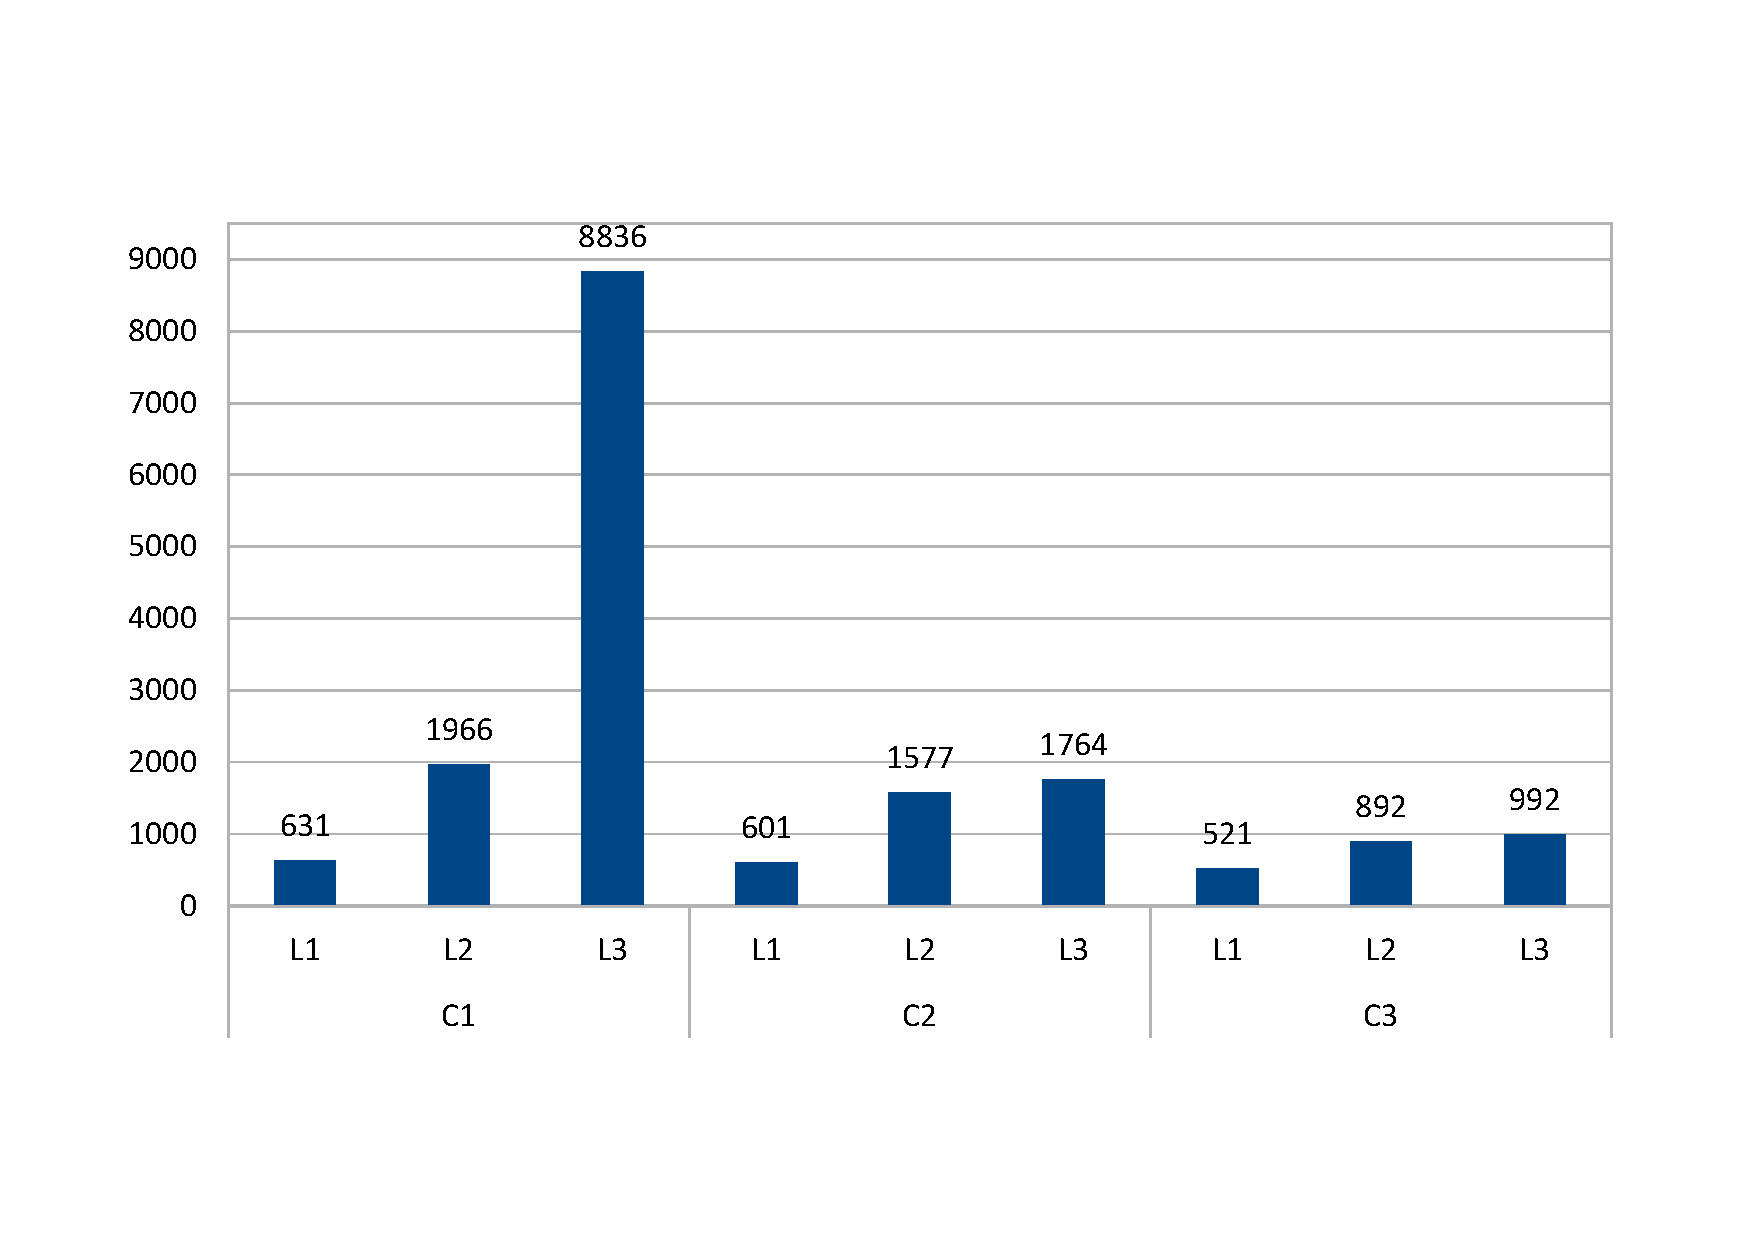
\includegraphics[width=0.9\textwidth,natwidth=200,natheight=150]{./fig/RTavg.pdf}
	\caption{The average response time for all configurations}
	\label{fig:rtavg}
\end{figure}

The test performed with the following loads: (L1) ten users request \emph{two} applications, (L2) ten users request \emph{four} applications and (L3) ten users request \emph{eight} applications. All three Loads run consecutively one hundred times each. Those Loads request applications, which have ten execution rows pulled from the repository of applications models and executions, and about one hundred queries to the social network database. In this experiment we kept the following components of the system constant: the Elgg front-end Apache2 server, the social network database, and the CDO server - client communication but we increased the number of memcached nodes.
Figure~\ref{fig:rtavg} shows the  average response time (RT) in milliseconds (ms) with the following system configuration(C): (C1) no memcached node, (C2) one memcached node and (C3) two memcached nodes have added to the system architecture.

Going from C1 to C3 and specifically for L3, the RT is reduced by 80,4\% in C2 and by 88,78\% in C3. As the Figure~\ref{fig:rtavg} shows, in the first configuration C1, the L3 takes 8836 ms, an RT which is definitely prohibitive for web applications. Introducing more memcached nodes at C2 and C3 the RT is decreased dramatically at 1764 ms at L2 and at 992 ms at L3. Going from C1 to C2, the 80,4\% reduction of RT is due to the introduction of memcached node and bypassed the steps I - V, which are mentioned previously. Going from C2 to C3, the RT reduced by a factor of 43,77\%. The reduction of RT is achieved by adding more memcached nodes, which results to more CPU cores introduced to the system, as described below.

\begin{figure}[h]
	\centering
	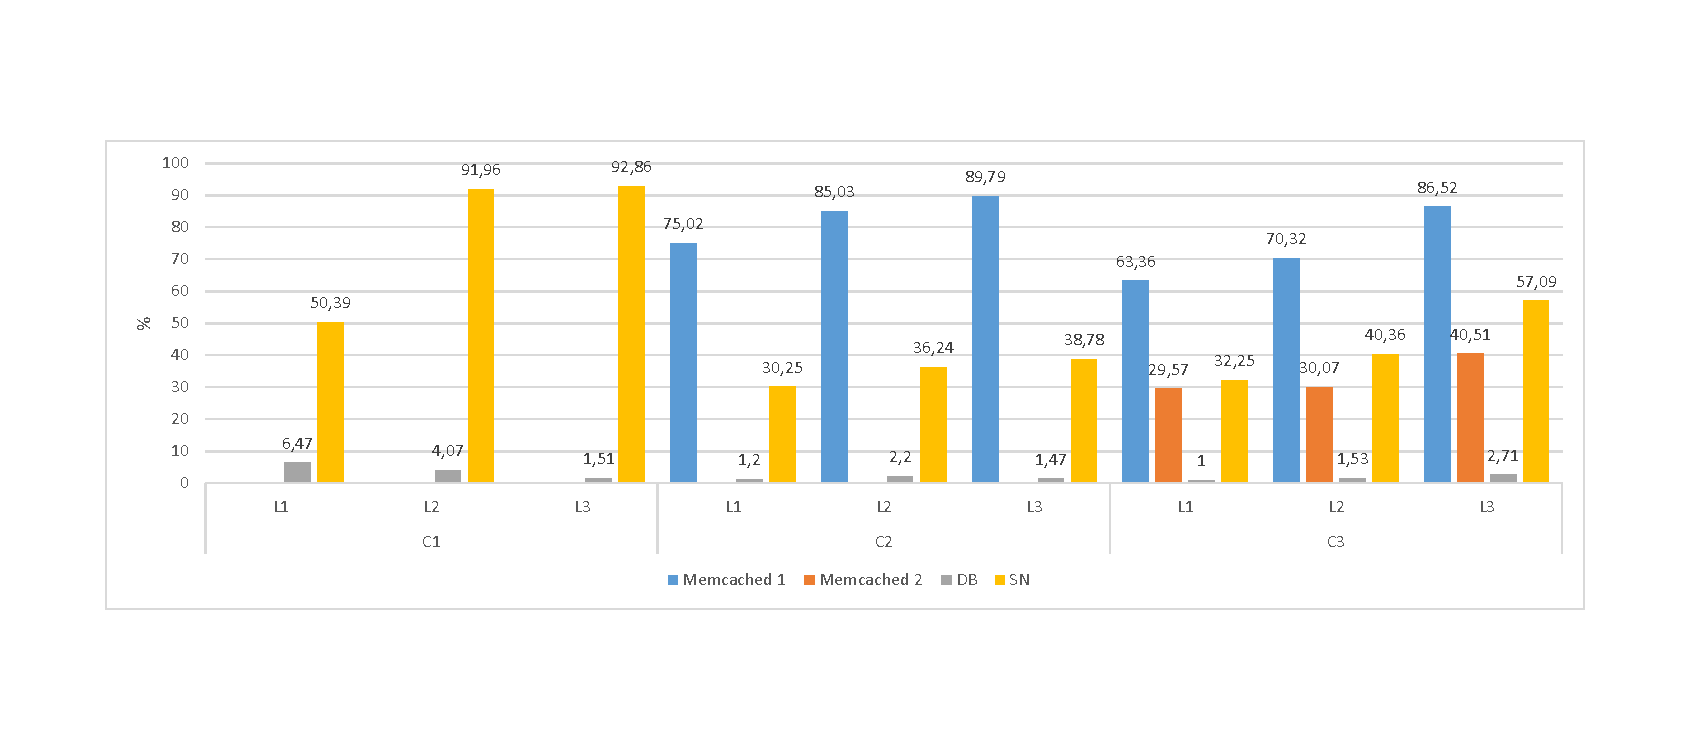
\includegraphics[width=1.1\textwidth]{./fig/UsageAVG.pdf} 
	\caption{The average CPU utilization for all components}
	\label{fig:cpuavg}
\end{figure}

The CPU utilization is measured using the sysstat tool~\cite{sysstat_url}. We measured the CPU utilization for all the VMs running the experiment. The information about the VM resources is listed in Table~\ref{vms_resources}. The social network engine and the CDO Client were running at t1.micro instance. The MySQL (repositories) and the CDO Server were running at m1.xlarge. The average CPU utilization is shown in Figure~\ref{fig:cpuavg}. At the simple configuration C1, even in small loads such as L1, the SN engine reached 50,39\% CPU utilization. In the medium load L2 and big load L3 the SN Engine is kneeled down to 91,96\% and 92,86\%. This big consumption of CPU was due to all the initialization process that Elgg social network engine has to do for each request and due to CDO server queries. Also, the CPU bottleneck of Elgg engine is responsible for the slow response time.

Moving from configuration C1 to C2, the CPU consumption went to memcached node. Thus, the social network engine was de-congested and the RT improved. However, for the big load L3 the memcached node reached 89,79\%. To solve memcached CPU overhead, one more memcached node was added at configuration C3. This second memcached node shared the CPU overhead with the first memcached node and the RT improved furthermore. 

For all three loads at C3, the first memcached node had more CPU utilization from the second by an approximately factor of 2,2. This difference between the two memcached nodes appeared due to the first node storing more popular key-value pairs than the other.

\begin{table}[]
\centering
\begin{tabular}{|l|l|}
\hline
 Component &  VM type \\ \hline
 SN engine, CDO client &  t1.micro \\ \hline
 memcached &  t1.micro \\ \hline
 repositories, CDO Server &  m1.xlarge \\ \hline
 jmeter &  m1.large \\ \hline
\end{tabular}
\caption{VM resources}
\label{vms_resources}
\end{table}

\subsection{Scaling the Elgg engine tier}

\begin{figure}[h]
	\centering
	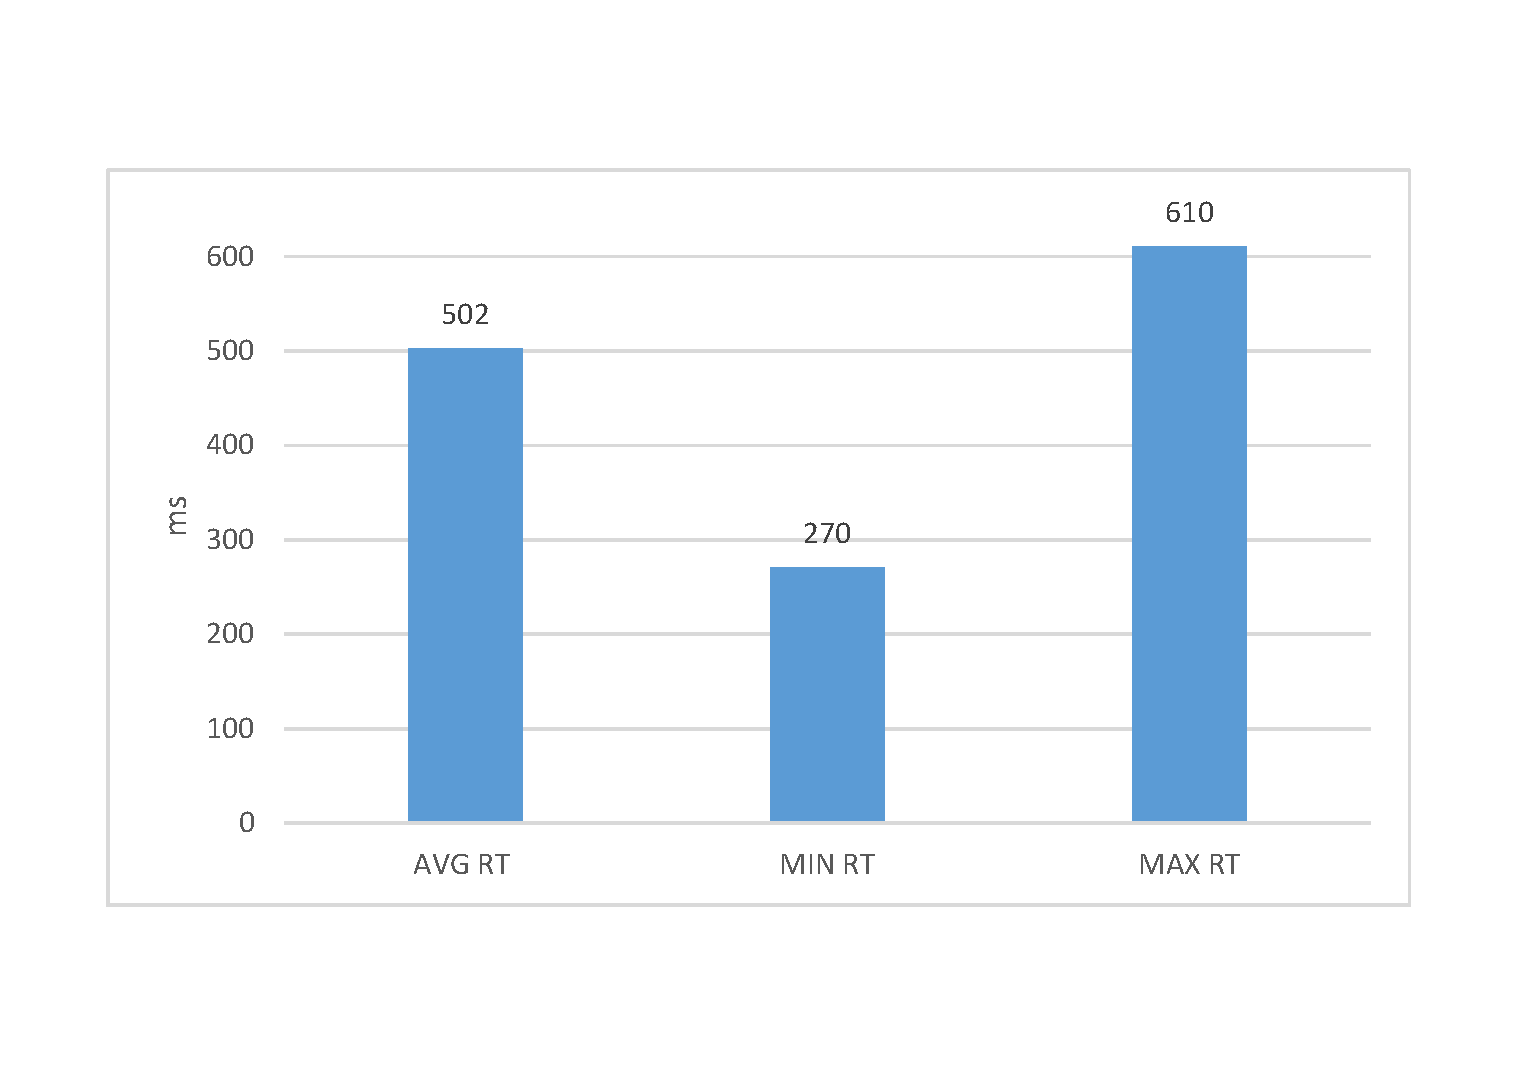
\includegraphics[width=0.8\textwidth,natwidth=200,natheight=150]{./fig/RT2SN.pdf}
	\caption{The response time for two social network engines}
	\label{fig:rt2SN}
\end{figure}

\begin{figure}[h]
	\caption{The CPU utilization for two social network engines}
	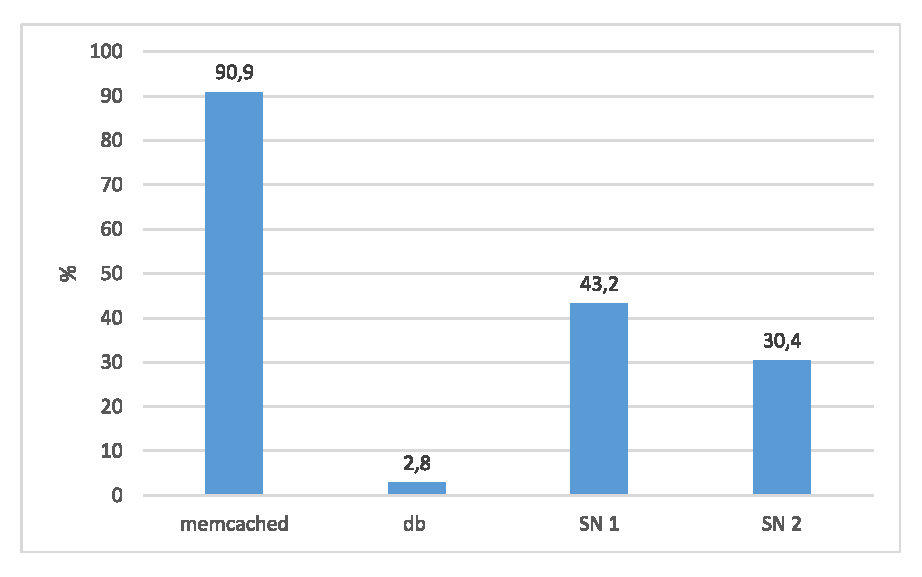
\includegraphics[width=0.8\textwidth,natwidth=200,natheight=150]{./fig/Usage2SN.pdf}
	\centering
	\label{fig:cpu2SNavg}
\end{figure}

This section evaluates the horizontal scale of social network engine as described in Section~\ref{sec:engine_scale}. A memcached node was living between the social networking engines and the back end system. The VM resources were kept the same as in the previous experiment and are shown in Table~\ref{vms_resources}. One more social networking engine instance was added with the same type as former SN engine. 

So, the system architecture now consists of two social networking engines as front-end. At the back-end of the system we have: (1) one memcached node and (2) the CDO client - server, the social network database and the CDO repository. The two SN engines are deployed to a dedicated VM each. Furthermore, each SN engine has its own CDO client deployed with them. The memcached node is deployed on its own VM and the CDO Server, the social network database and the CDO repository are deployed on the same VM.

The Figure~\ref{fig:cpu2SNavg} shows the average CPU utilization for the memcached, the MySQL database (db) and the two SN Engines (SN1, SN2). The load for this experiment is the same as the previous load L3, which means we have ten users that request \emph{eight} applications for one hundred times consecutively. The first SN engine has 43,2\% CPU usage and the second one has 12,8\% less. This difference is due to the first instance being deployed together with the NFS server and Apache Zookeeper on the same VM. 

With only one SN engine the CPU utilization was 57,09\% and now with two SN engines the CPU utilization is reduced to 43,2\%. This reduction is due to the requests being distributed to two instances instead of the only one instance. The CPU utilization of the memcached node increased, but this can be solved by introducing more memcached nodes as the previous section describes. Furthermore, we can introduce more SN engines to support more heavy loads.

Since the load from one SN engine is now distributed to two SN engines instances, the response time improved for the Load 3, as shown in the Figure~\ref{fig:rt2SN} compared to the previous test-bench. The best achieved RT of previous architecture was 992 ms and with this architecture it reduced to 502 ms.

We can combine the two architectures together, meaning that we have more than one SN Engine and more than one memcached to support as many loads as we want.

\section{Topic classification}
\label{sec:nlp_evaluation}
This section evaluates the topic classification tool described in Section~\ref{sec:natural_implementation}. The evaluated topic classifier had four different classes or, according to StackOverflow (SO) dialect, six tags, as are shown in Table~\ref{table:nlp_eval}. Those classes are: (1)~\emph{architecture and design}, (2)~\emph{scalability}, (3)~\emph{performance and optimization} and (4)~\emph{deployment}. This means that a new question can be classified in one of the previous four classes.

The~\emph{architecture} tag and the~\emph{design} tag comprised one class in our topic classifier because those two tags have similar meaning for the users of SO. Also, the~\emph{performance} and~\emph{optimization} tags defined another class for the same reason.

For the testing set, thirty questions from StackOverflow were used per class, in order to measure the topic classification accuracy. Those questions were different from the training set and were the most up-voted questions during the specific time period that this experiment was carried out. Each row in Table~\ref{table:nlp_eval} shows a class as classified by StackOverflow users, and each column shows how our classifier classifies the question. For example, twenty nine questions about~\emph{architecture and design} were classified correctly, and only one was wrongly classified as \emph{performance \& optimization}. The misclassification however, was not an error of our classifier. 

For the evaluation process, the title and the body of the questions are used to determine their class. The title of the question is very helpful for the determination of the class because in same cases the SO users ask their questions in the title of the question and poses only code in the body of the question along with a small explanation about the code. So, without the title of the question the topic classifier can not determine correctly the class of the question. Furthermore, the code which was existing in the body of the questions was removed in order to not misguide our topic classifier.

Furthermore, the classes used in this evaluation have similar meaning to each other. SO users sometimes use those tags without knowing their meaning. Also, the scalability tag is too broad and can have keywords from the architecture and design class.

This shows that our tool can further be used by StackOverflow to mark new questions that are wrongly tagged or misguided. There is a trend among StackOverflow users to add as many tags as they can in order to attract the attention of other users, increase the views of their question and finally get their answers.  

The true positive, which means a document is recognized in the correct class, according the Table~\ref{table:nlp_eval} is 96. The false positive, which means a document is not correctly recognized, of this topic classification evaluation is 24. According to those precision metrics the accuracy or sensitivity of our topic classifier for this specific experiment is 80\%.

For future work, this evaluation can be extended by imported questions and answers for other information repositories which have more similar terns to our social networking platform and with classes with different meaning to each other.

\newcommand{\specialcell}[2][c]{%
  \begin{tabular}[#1]{@{}c@{}}#2\end{tabular}}
  
\begin{table}[]
\centering
\label{my-label}
\begin{tabular}{|l|l|l|l|l|}
\hline
class / class & \specialcell{architecture\\ \& design} & \specialcell{performance \\ \& optimization} & deployment  & scalability \\ \hline
\specialcell{architecture\\ \& design}  & \textbf{29}  & 0            & 0           & 1           \\ \hline
\specialcell{performance \\ \& optimization}  & 2            & \textbf{23}  & 0           & 5           \\ \hline
deployment    & 6            & 0            & \textbf{22} & 2           \\ \hline
scalability   & 7            & 0            & 1           & \textbf{22} \\ \hline
\end{tabular}
\caption{Evaluation of topic classification}
\label{table:nlp_eval}
\end{table}

\section{Requirements and user interface}
\label{eval_ui}
The user interface (UI) of our social networking platform\footnote{The user interface (UI) design and usability evaluation was the result of a collaboration with the Human-Computer Interaction (HCI) laboratory of ICS-FORTH~\cite{magoutis2015design}.} is designed through an iterative process of several expert-based evaluations carried out in group sessions. To obtain additional feedback from non-experts, three additional user-based evaluation experiments were designed and carried out involving potential users and presented in detail in~\cite{magoutis2015design}. 

The author collaborated in the expert-based evaluations sessions focusing on the platform user interface design.  He contributed in the UI usability evaluations through the implementation of the platform, and took active part by interviewing some of the participants in the third evaluation experiment.  

The first experiment, carried out by Flexiant Ltd. aimed at assessing the overall look and feel of the network, the navigation mechanisms, as well as the design of fundamental functionality.
The second evaluation experiment, carried out by a FORTH team consisting of HCI and CARV laboratory members, aimed to collect subjective results rather than performance metrics. It involved another set of 12 users who, after a brief introduction to the available facilities, were asked to use the interactive prototype~\cite{Virzi1996} using the free exploration method of the Thinking Aloud protocol~\cite{jordan1998introduction} and fill-in a questionnaire in order to rate and comment their experience. 

The third evaluation experiment involved 15 participants guided through the interactive prototype of our social networking platform using specific scenarios. They were interviewed on their requirements and feedback following a semi-structured interview approach [84]. The evaluation session was carried out via Skype. Participants were recruited through European companies and organizations associated with the PaaSage EU project~\cite{paasage}. They were either developers or operations staff, thus within the target user groups of our social networking platform. Participants were not users of the  platform; some however were familiar with the project’s goals and objectives. Before the experiment, each participant was requested to fill-in a background information form and was sent an informed consent form, explaining all the recording and anonymity-ensuring procedures. 

\begin{figure}[h]
	\centering
	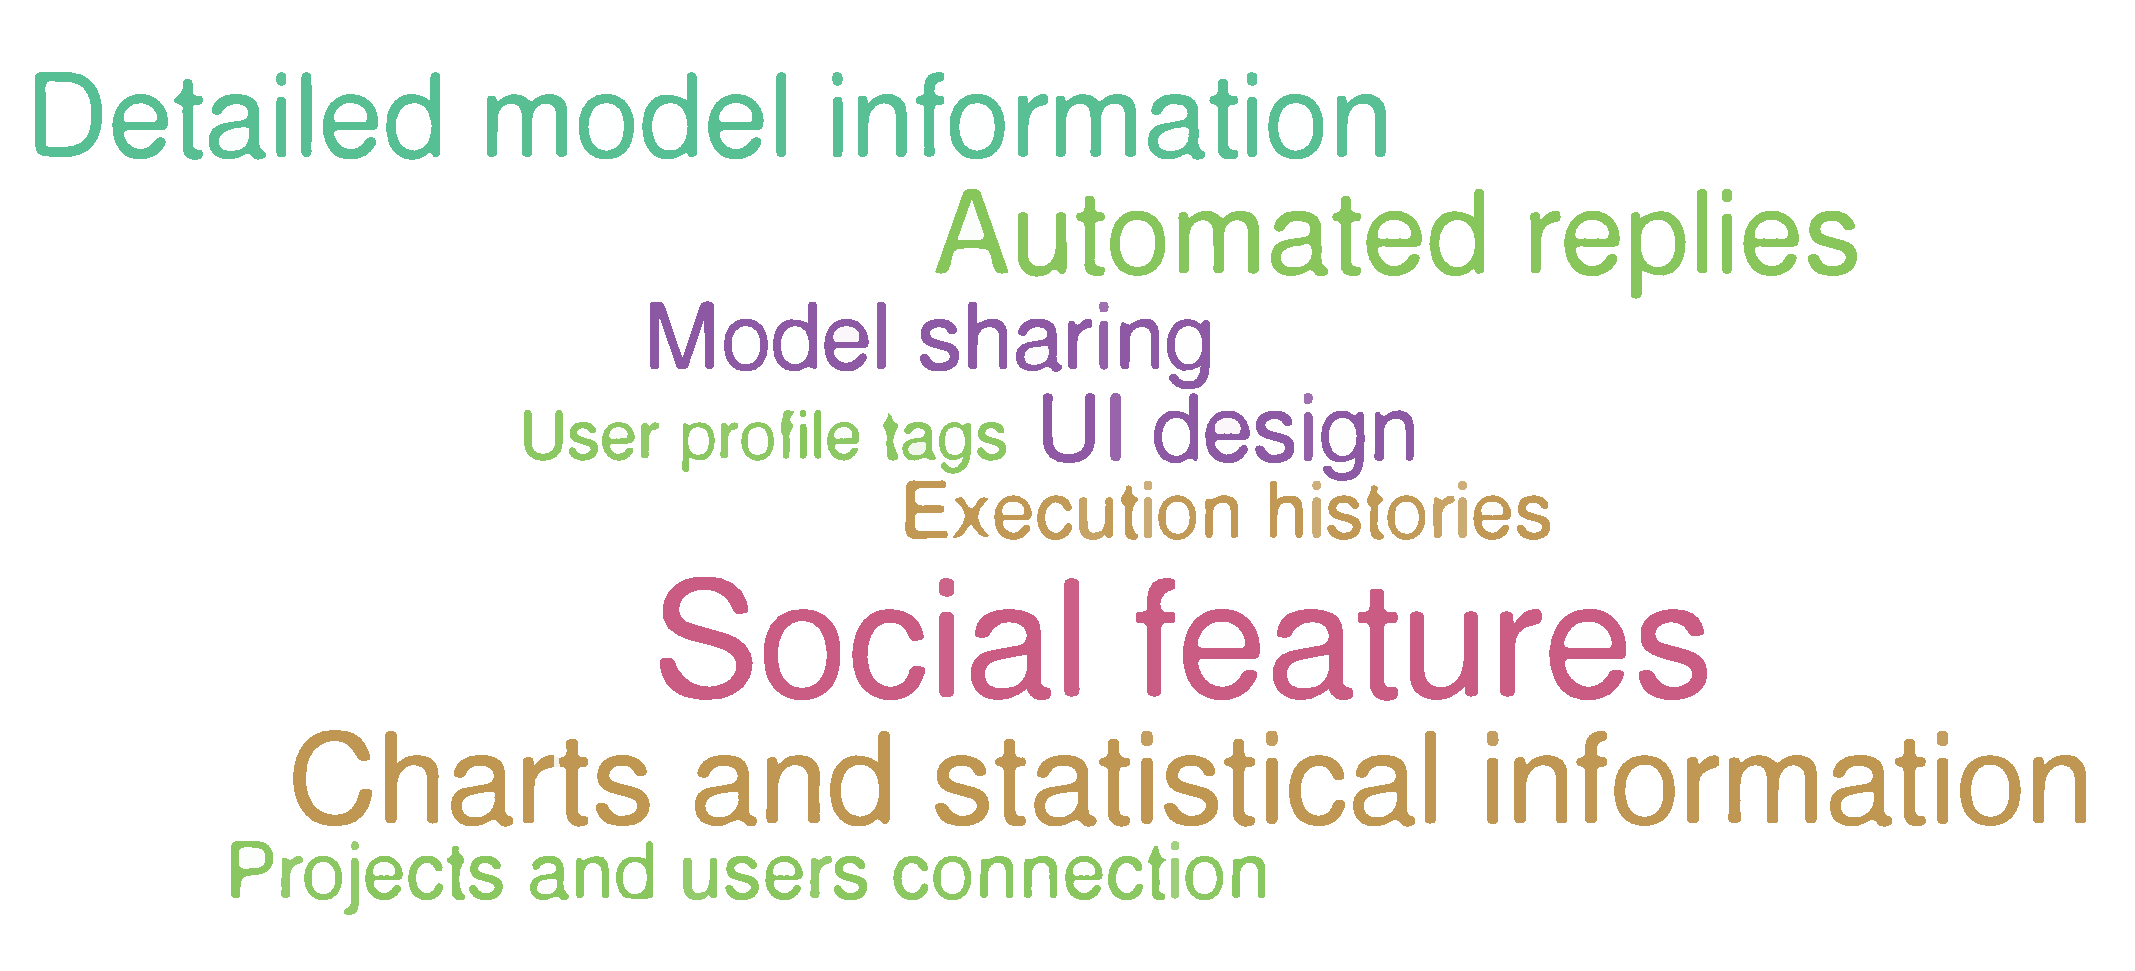
\includegraphics[width=1\textwidth,natwidth=200,natheight=150]{./fig/most-liked.pdf}
	\caption{Features that were mostly liked by the users}
	\label{fig:most-liked}
\end{figure}

Users in the third experiment were asked to identify up to three most-liked and three most-disliked features. Most-liked features presented in Figure~\ref{fig:most-liked} included: the employment of social features in a development environment; the use of charts and statistical information to represent data; the detailed model information that could be retrieved and the model execution histories; the automatically-generated hints provided by the network as replies in discussion topics; the concept of sharing one’s models; the overall UI design; the direct connection between projects and users, and the user profile tags that allowed them to find users that would be interesting to connect with.

Those user interface evaluation experiments show that a platform that couples social networking features in community-building activities with DevOps requirements for application deployment, analyses of the execution histories, and automatically generated hints based on data analysis, is a helpful tool that people would like to use. Furthermore, those evaluation experiments show that the design and the implementation of our social networking platform was functional and easy to use.